\section{Results}
\label{sec:results}

We report the confirmatory test first, because it is the only part of the study designed to support a claim, and then the exploratory pilot results that contextualise it. Unless stated otherwise, intervals are paired 95\% bootstrap intervals over questions, and differences are stated as the first-named representation minus the second-named one.

\subsection{Confirmatory test of the primary contrasts}

Table~\ref{tab:confirmatory} reports the six pre-specified tests on the disjoint confirmatory sample of 1{,}744 MuSiQue and 3{,}232 2WikiMultiHopQA questions. All 44{,}784 records were generated without errors, with information equivalence verified for every question.

One of the six tests rejects the null hypothesis after Holm correction. On 2WikiMultiHopQA, presenting the gold passages as sentence items (R1) instead of passages (R0) lowers exact match by 0.017 (95\% CI $[-0.029, -0.005]$, $p_{\text{Holm}}=0.018$); the paired coverage difference is $-0.052$. On MuSiQue the same contrast is $-0.001$ $[-0.014, +0.014]$, and its 90\% interval lies inside the pre-specified equivalence margin of $\pm0.02$.

Neither structural contrast is significant on either dataset. Graph-derived ordering (R5$-$R1) gives $-0.011$ $[-0.026, +0.003]$ on MuSiQue and $-0.008$ $[-0.018, +0.002]$ on 2WikiMultiHopQA, and explicit relation lines at a fixed order (R4$-$R5) give $+0.010$ $[-0.003, +0.024]$ and $+0.006$ $[-0.002, +0.015]$. On 2WikiMultiHopQA both structural contrasts are equivalent to zero within $\pm0.02$. On MuSiQue neither interval excludes zero, but neither lies inside the margin either, so we can only call them inconclusive.

Two features of the data qualify the structural contrasts. First, many pairs are byte-identical: R5 equals R1 for 1{,}858 of 3{,}232 2WikiMultiHopQA questions and 522 of 1{,}744 MuSiQue questions, and R4 equals R5 for the 879 2WikiMultiHopQA questions without derived edges. Restricted to the pairs whose evidence differs, the estimates are $-0.019$ (2Wiki, R5$-$R1), $-0.016$ (MuSiQue, R5$-$R1) and $+0.008$ (2Wiki, R4$-$R5). Second, all structure is derived from dataset annotations, not verified by humans, so a null result concerns derived structure of this quality.

\begin{table*}[t]
\centering
\footnotesize
\begin{tabular}{@{}llrrlrrrrrrl@{}}
\toprule
Data & Contrast & $n$ & $\Delta$EM & 95\% CI & $p$ & $p_{\text{Holm}}$ & +/$-$ & Ident. & Inform. $\Delta$ & $\Delta$Cov. & Equiv. \\
\midrule
MuSiQue & R1$-$R0 & 1744 & -0.001 & [-0.014, +0.014] & 0.974 & 0.974 & 70/71 & 3 & -0.001 & +0.009 & yes \\
MuSiQue & R5$-$R1 & 1744 & -0.011 & [-0.026, +0.003] & 0.122 & 0.535 & 68/88 & 522 & -0.016 & +0.003 & no \\
MuSiQue & R4$-$R5 & 1744 & +0.010 & [-0.003, +0.024] & 0.117 & 0.535 & 75/57 & 0 & +0.010 & +0.004 & no \\
2Wiki & R1$-$R0 & 3232 & -0.017 & [-0.029, -0.005] & 0.003 & 0.018 & 185/239 & 44 & -0.017 & -0.052 & no \\
2Wiki & R5$-$R1 & 3232 & -0.008 & [-0.018, +0.002] & 0.107 & 0.535 & 126/152 & 1858 & -0.019 & -0.012 & yes \\
2Wiki & R4$-$R5 & 3232 & +0.006 & [-0.002, +0.015] & 0.174 & 0.535 & 103/84 & 879 & +0.008 & -0.011 & yes \\
\bottomrule
\end{tabular}
\caption{Confirmatory test of the six pre-specified primary contrasts (Protocol~A, EM, disjoint sample; \texttt{docs/CONFIRMATORY\_PROTOCOL.md}). $p$: two-sided paired bootstrap; $p_{\text{Holm}}$: Holm-adjusted over the six tests. Equiv.: 90\% CI inside $\pm0.02$ (pre-specified secondary check). Source: \texttt{F\_exp1\_contrasts.csv}.}
\label{tab:confirmatory}
\end{table*}


\subsection{Where the confirmed effect comes from}

Table~\ref{tab:decomposition-main} splits each paired difference according to which of the two conditions produced an answer. This decomposition was added after we saw the confirmatory result and is exploratory. For R1$-$R0 on 2WikiMultiHopQA, the questions that both representations answered contribute $+0.001$; the effect comes almost entirely from questions answered under only one representation, where the model abstained under the sentence format on 250 questions that it answered under passages, against 81 in the other direction.
In other words, for this generator the sentence format did not make answered questions less accurate. It made the model more likely to reply \emph{insufficient evidence} when given exactly the same facts. Abstention is pervasive in general: with complete gold evidence, 710 of 1{,}744 MuSiQue questions and 529 of 3{,}232 2WikiMultiHopQA questions are answered under neither R0 nor R1.

\input{tables/tab_decomposition_main}

\subsection{Secondary contrasts on the confirmatory sample}

The confirmatory run also generated the secondary representations, whose contrasts were pre-specified as secondary and are therefore descriptive (Figure~\ref{fig:forest}; Table~\ref{tab:confirm-secondary} in Appendix~\ref{app:tables}).

Replacing derived relations with model-predicted relations (R4P$-$R4) lowers exact match on both datasets: by 0.036 $[-0.045, -0.027]$ on 2WikiMultiHopQA and 0.045 $[-0.060, -0.030]$ on MuSiQue, with coverage differences of $-0.061$ and $-0.089$. The effect of shuffling the sentence items (R2$-$R1) depends on the dataset: $-0.024$ $[-0.036, -0.012]$ on 2WikiMultiHopQA but $+0.013$ $[-0.001, +0.028]$ on MuSiQue. Grouping items under reasoning steps (R3$-$R5) makes no detectable difference ($-0.004$ and $-0.007$).

\begin{figure*}[t]
\centering
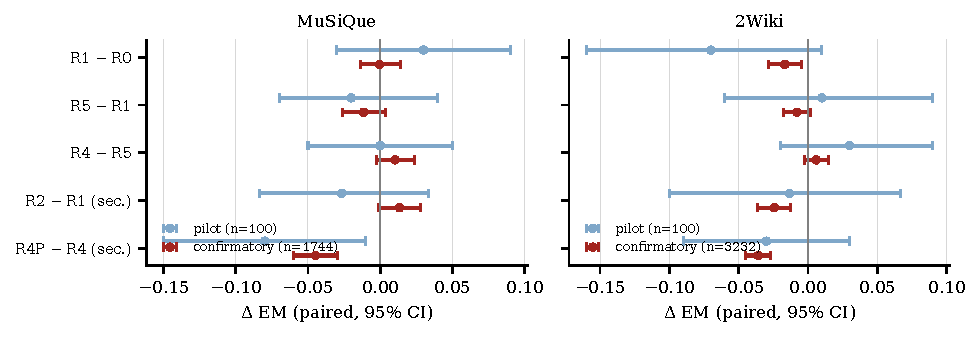
\includegraphics[width=0.92\textwidth]{figures/fig5_contrasts_pilot_vs_confirmatory.pdf}
\caption{Protocol~A contrasts in the exploratory pilot ($n$=100 per dataset) and on the disjoint confirmatory sample. The pilot estimate of R1$-$R0 on 2WikiMultiHopQA ($-0.07$) overstated the confirmed effect ($-0.017$). Contrasts marked \emph{sec.} are secondary.}
\label{fig:forest}
\end{figure*}


\subsection{Exploratory pilot results}

Protocol~B, the retrieved-evidence baselines and the perturbations were run only on the exploratory pilot ($n=100$ per primary dataset). Appendix~\ref{app:pilot} gives the details and Appendix~\ref{app:tables} the tables. \emph{Budget (Protocol~B).} Under a budget equal to the content tokens of the fact set, with each representation keeping as much of the shared ranking as it can afford, R0 keeps 0.83 (2WikiMultiHopQA) and 0.81 (MuSiQue) of the facts, against 0.62--0.65 for R1, R4 and R5, whose identifiers, titles and relation lines cost 2.5 to 4 times as many overhead tokens. The answer string consequently remains in 0.85 of R0 blocks on 2WikiMultiHopQA but only 0.64--0.66 of the others; the accuracy differences are smaller than these losses and inconclusive at this $n$. \emph{Retrieved evidence (Experiment~0).} Extracted claims and predicted paths are indistinguishable from reranked passages in exact match, at about three times the tokens. Our EG-RAG reconstruction, at a similar token count to reranked passages, is less accurate ($-0.15$ on 2WikiMultiHopQA and $-0.09$ on MuSiQue), because its budgeted selection keeps the answer string less often and it abstains more. \emph{Perturbations (Experiment~2).} Removing required facts mainly raises abstention, hard distractors lower exact match in every QA cell (by up to 0.16), and retyping 40\% of the derived relations lowers 2WikiMultiHopQA exact match by 0.10 $[-0.18, -0.01]$. Reordering and stripping titles have small effects of inconsistent sign.
